% This is samplepaper.tex, a sample chapter demonstrating the
% LLNCS macro package for Springer Computer Science proceedings;
% Version 2.21 of 2022/01/12
%
\documentclass[runningheads]{llncs}
%
\usepackage[T1]{fontenc}
% T1 fonts will be used to generate the final print and online PDFs,
% so please use T1 fonts in your manuscript whenever possible.
% Other font encondings may result in incorrect characters.
%
\usepackage{graphicx}
% Used for displaying a sample figure. If possible, figure files should
% be included in EPS format.
%
% If you use the hyperref package, please uncomment the following two lines
% to display URLs in blue roman font according to Springer's eBook style:
%\usepackage{color}
%\renewcommand\UrlFont{\color{blue}\rmfamily}
%\urlstyle{rm}
%
\begin{document}
%
\title{Difficulty-Aware Adaptive Test-Time Compute: A Depth-First Joint Allocation Approach}
\titlerunning{Depth-First Joint Allocation for Small Reasoning Models}
%
%\titlerunning{Abbreviated paper title}
% If the paper title is too long for the running head, you can set
% an abbreviated paper title here
%
\author{Dinh-Hong Vu\inst{1}\orcidID{0000-0001-8513-3942} \and
The-Tai Phung\inst{2} \and
Thai-Son Bui\inst{3}}
%
\authorrunning{Dinh-Hong Vu, The-Tai Phung and Thai-Son Bui}
% First names are abbreviated in the running head.
% If there are more than two authors, 'et al.' is used.
%
\institute{Natural Language Processing and Knowledge Discovery Research Group, Faculty of Information Technology, Ton Duc Thang University, Ho Chi Minh City, Vietnam\\
\email{vudinhhong@tdtu.edu.vn}
\and 
Faculty of Information Technology, Ton Duc Thang University, Ho Chi Minh City, Vietnam\\
\email{\{52300059, 52300058\}@student.tdtu.edu.vn}}
%
\maketitle              % typeset the header of the contribution
%
\begin{abstract}
Reasoning-oriented language models can improve problem-solving performance by spending additional test-time compute, for example, by generating longer reasoning trajectories or sampling multiple independent reasoning paths. However, most existing inference strategies either allocate a fixed compute budget to all inputs or adapt only a single dimension of computation, which may waste resources on easy problems while still under-serving harder ones. To address this limitation, we propose a Joint Breadth–Depth Adaptive Test-Time Compute framework for Small Reasoning Models, where breadth controls the number of independent reasoning samples and depth controls the generation budget assigned to each sample. Rather than treating these two forms of computation independently, the framework jointly reasons about how inference resources should be distributed on a per-problem basis. Its core design follows a depth-first, selective-breadth principle: sufficient generation budget is allocated to obtain a usable reasoning trajectory, while additional sampling is introduced only when extra reasoning paths are expected to provide meaningful benefit. A lightweight controller is used to estimate the required compute configuration from inexpensive input-level and early-inference signals, with the goal of minimizing unnecessary computation while preserving reasoning quality. The framework is evaluated across multiple reasoning models and benchmark datasets against fixed-budget, depth-only, breadth-only, and adaptive inference baselines using final-answer accuracy, realized token usage, latency, and accuracy–compute trade-offs. The study aims to determine whether joint allocation of reasoning breadth and generation depth can provide a more efficient and generalizable strategy for test-time scaling than conventional single-axis approaches.

\keywords{Adaptive Test-Time Compute, Small Reasoning Models, Joint Breadth–Depth Allocation, Adaptive Inference, Reasoning Efficiency, Compute Allocation, Lightweight Controller.}
\end{abstract}
%
%
%
\section{Introduction}
\subsection{A Subsection Sample}
Please note that the first paragraph of a section or subsection is
not indented. The first paragraph that follows a table, figure,
equation etc. does not need an indent, either.

Subsequent paragraphs, however, are indented.

\subsubsection{Sample Heading (Third Level)} Only two levels of
headings should be numbered. Lower level headings remain unnumbered;
they are formatted as run-in headings.

\paragraph{Sample Heading (Fourth Level)}
The contribution should contain no more than four levels of
headings. Table~\ref{tab1} gives a summary of all heading levels.

\begin{table}
\caption{Table captions should be placed above the
tables.}\label{tab1}
\begin{tabular}{|l|l|l|}
\hline
Heading level &  Example & Font size and style\\
\hline
Title (centered) &  {\Large\bfseries Lecture Notes} & 14 point, bold\\
1st-level heading &  {\large\bfseries 1 Introduction} & 12 point, bold\\
2nd-level heading & {\bfseries 2.1 Printing Area} & 10 point, bold\\
3rd-level heading & {\bfseries Run-in Heading in Bold.} Text follows & 10 point, bold\\
4th-level heading & {\itshape Lowest Level Heading.} Text follows & 10 point, italic\\
\hline
\end{tabular}
\end{table}


\noindent Displayed equations are centered and set on a separate
line.
\begin{equation}
x + y = z
\end{equation}
Please try to avoid rasterized images for line-art diagrams and
schemas. Whenever possible, use vector graphics instead (see
Fig.~\ref{fig1}).

\begin{figure}
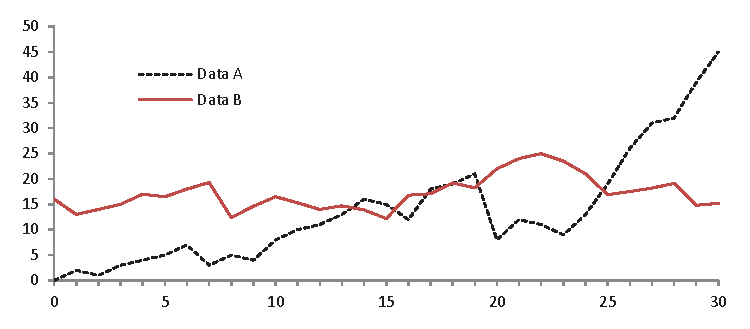
\includegraphics[width=\textwidth]{fig1.eps}
\caption{A figure caption is always placed below the illustration.
Please note that short captions are centered, while long ones are
justified by the macro package automatically.} \label{fig1}
\end{figure}

\begin{theorem}
This is a sample theorem. The run-in heading is set in bold, while
the following text appears in italics. Definitions, lemmas,
propositions, and corollaries are styled the same way.
\end{theorem}
%
% the environments 'definition', 'lemma', 'proposition', 'corollary',
% 'remark', and 'example' are defined in the LLNCS documentclass as well.
%
\begin{proof}
Proofs, examples, and remarks have the initial word in italics,
while the following text appears in normal font.
\end{proof}
For citations of references, we prefer the use of square brackets
and consecutive numbers. Citations using labels or the author/year
convention are also acceptable. The following bibliography provides
a sample reference list with entries for journal
articles~\cite{ref_article1}, an LNCS chapter~\cite{ref_lncs1}, a
book~\cite{ref_book1}, proceedings without editors~\cite{ref_proc1},
and a homepage~\cite{ref_url1}. Multiple citations are grouped
\cite{ref_article1,ref_lncs1,ref_book1},
\cite{ref_article1,ref_book1,ref_proc1,ref_url1}.

\begin{credits}
\subsubsection{\ackname} A bold run-in heading in small font size at the end of the paper is
used for general acknowledgments, for example: This study was funded
by X (grant number Y).

\subsubsection{\discintname}
It is now necessary to declare any competing interests or to specifically
state that the authors have no competing interests. Please place the
statement with a bold run-in heading in small font size beneath the
(optional) acknowledgments\footnote{If EquinOCS, our proceedings submission
system, is used, then the disclaimer can be provided directly in the system.},
for example: The authors have no competing interests to declare that are
relevant to the content of this article. Or: Author A has received research
grants from Company W. Author B has received a speaker honorarium from
Company X and owns stock in Company Y. Author C is a member of committee Z.
\end{credits}
%
% ---- Bibliography ----
%
% BibTeX users should specify bibliography style 'splncs04'.
% References will then be sorted and formatted in the correct style.
%
% \bibliographystyle{splncs04}
% \bibliography{mybibliography}
%
\begin{thebibliography}{8}
\bibitem{ref_article1}
Author, F.: Article title. Journal \textbf{2}(5), 99--110 (2016)

\bibitem{ref_lncs1}
Author, F., Author, S.: Title of a proceedings paper. In: Editor,
F., Editor, S. (eds.) CONFERENCE 2016, LNCS, vol. 9999, pp. 1--13.
Springer, Heidelberg (2016). \doi{10.10007/1234567890}

\bibitem{ref_book1}
Author, F., Author, S., Author, T.: Book title. 2nd edn. Publisher,
Location (1999)

\bibitem{ref_proc1}
Author, A.-B.: Contribution title. In: 9th International Proceedings
on Proceedings, pp. 1--2. Publisher, Location (2010)

\bibitem{ref_url1}
LNCS Homepage, \url{http://www.springer.com/lncs}, last accessed 2023/10/25
\end{thebibliography}
\end{document}
